\documentclass[10pt]{article}
\usepackage[top=50pt,bottom=50pt,left=48pt,right=46pt]{geometry}
\usepackage{color}
\usepackage[utf8]{inputenc}
\usepackage{float}
\usepackage[T1]{fontenc}
% \usepackage{indentfirst}
\usepackage{amsmath}
\usepackage{graphicx}
\usepackage{hyperref} 
% used for enumerate based on different symbols
% \begin{enumerate}[(a)] e.g.
\usepackage[shortlabels]{enumitem}

% beautifully indenting an environment
% \begin{addmargin}[1em]{2em}
% \end{addmargin}
% args: left margin, right margin
\usepackage{scrextend}

% for centered p columns in tabular environment
% \begin{tabular}{|P{2cm}|P{40mm}|P{4cm}|}
\usepackage{array}
\newcolumntype{P}[1]{>{\centering\arraybackslash}p{#1}}
\newcolumntype{M}[1]{>{\centering\arraybackslash}m{#1}}

% set paragraph indent to 0
% if you want to indent some paragraph, use \indentfirst command in front of them
\setlength{\parindent}{0pt}
\newcommand{\forceindent}{\leavevmode{\parindent=1em\indent}}


% for scaling a tabular table
\usepackage{graphicx}
\usepackage{grffile}


% for comment block
\usepackage{verbatim}

% for debug purposes
% \usepackage{showframe}

% for setting section start value
\setcounter{section}{6}

% for code writing
% \begin{lstlisting} code here \end{lstlisting}
\usepackage{listings}
\lstset{
	% numbers=left,
	breaklines=true,
	tabsize=2,
	literate={\ \ }{{\ }}1,
%	language=C,
	basicstyle=\footnotesize\ttfamily, 
	stepnumber=1,
%	aboveskip=-10pt,
}



\newcommand{\indentitem}{\setlength\itemindent{25pt}}
\graphicspath{ {screenshots/} }



% Title Page
\title{Implementation of Databases \\ ~~~ \\ Assignment 6 \\ ~~~ \\ }
\author{
	Participants:\\
	(sorted in last name order)\\
	Ulfet CETIN\\ 
	Shreya KAR\\
	Samuel ROY\\	
}
\date{}

\newlength{\mytab}
\setlength{\mytab}{1em}

\begin{document}

	\maketitle
	
	\clearpage
	\subsection*{Exercise 6.1 (Cost Estimation using Spark)}
	
	Consider the Chinook database from Exercise 1.2 and the 5th Query Q5.
	
	\begin{enumerate}
		\item Install Spark 2.4. In Exercise 1.2 you have data stored in PostgreSQL database. Export the
		data from tables Track and InvoiceLine individually to CSV files. Load these two CSV
		files into Spark. Alternatively, you can also load the data frames directly from PostgreSQL.
		Provide your codes.\\
		
		We used Ubuntu 18.04 LTS, clean installation, for both PostgreSQL and Spark.\\
		Here is how we do it:
		
			\begin{itemize}
				\item PostgreSQL CSV Export
					
					
					
					\begin{enumerate}[1.]
						\item Install PostgreSQL using terminal:\\
						sudo apt update\\
						sudo apt install postgresql postgresql-contrib\\
						
						\item Connect to PostgreSQL, create DB named "chinook":\\
						sudo -u postgres psql\\
						(psql shell) CREATE DATABASE chinook OWNER postgres;\\
						(psql shell) \textbackslash c chinook\\
						
						\item Import data from Assignment 1.\\
						sudo -u postgres psql chinook < Chinook\_DB/Chinook\_PostgreSql.sql\\
						
						\item Export data from inside psql shell.\\
						\textbackslash COPY "Track" TO '/tmp/track.csv' WITH (FORMAT CSV, HEADER);\\
						\textbackslash COPY "InvoiceLine" TO '/tmp/invoiceline.csv' WITH (FORMAT CSV, HEADER);\\
						(the files put in tmp folder to not cause privilege errors, retrieved from that folder)\\
					\end{enumerate}
				
					\bigskip
					\begin{figure}[H]
						\centering
						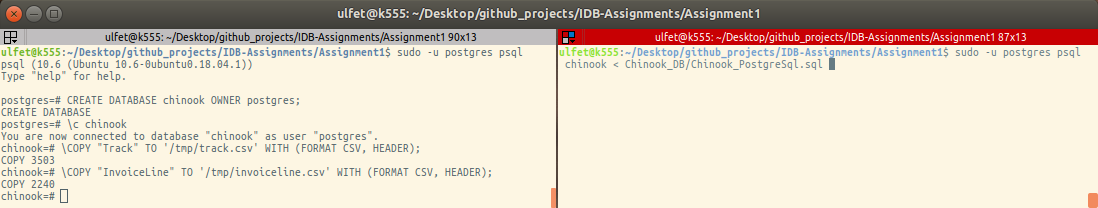
\includegraphics[scale=0.40]{postgres_csv.png}
						\caption{CSV Extraction via PostgreSQL}
						%\label{}
					\end{figure}
					\bigskip
				
				\bigskip
				
				\item Spark CSV Import
				
					\bigskip
					\begin{enumerate}[1.]
						\item Install Spark \& Java8 (required for Spark)\\
						sudo apt-add-repository ppa:webupd8team/java\\
						sudo apt-get update\\
						sudo apt-get install oracle-java8-installer\\
						https://spark.apache.org/downloads.html (download spark-2.4.0-bin-hadoop2.7.tgz)\\
						tar -xzvf spark-2.4.0-bin-hadoop2.7.tgz\\
						cd spark-2.4.0-bin-hadoop2.7/bin\\
						./pyspark (run pyspark once)\\
						
						\clearpage
						
						\item We would use Spark through Python.\\
						Here is the code for importing CSV files:\\
						
	\begin{lstlisting}
	# Spark is not installed system-wide
	# that is why findspark pip package is needed
	import findspark
	findspark.init()
	
	from pyspark.sql import SparkSession
	
	spark = SparkSession \
	.builder \
	.appName("IDB Assignment 6 Query Runner") \
	.getOrCreate()
	
	# read CSV files into DataFrames
	invLineDF = spark.read.csv("csv_files/invoiceline.csv",header=True);
	trackDF = spark.read.csv("csv_files/track.csv",header=True);
	
	# Displays the content of the DataFrame to stdout
	invLineDF.show(10)
	trackDF.show(10)
	\end{lstlisting}
						\bigskip
						\begin{figure}[H]
							\centering
							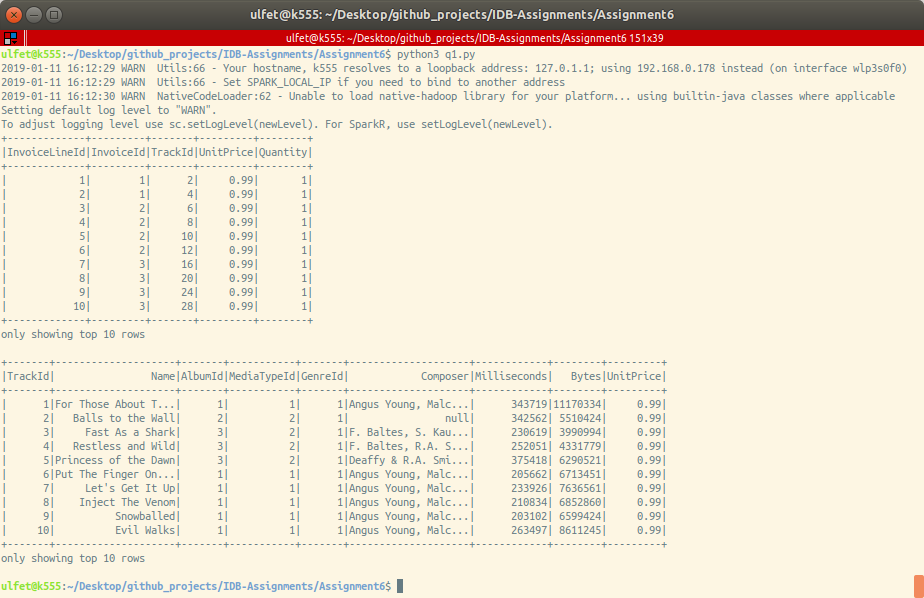
\includegraphics[scale=0.40]{spark_csv.png}
							\caption{CSV Importing in Spark}
							%\label{}
						\end{figure}
						\bigskip
					
						
					\end{enumerate}
					
			\end{itemize}
		
		
		\clearpage
		
		\item Run the previous query Q5 from Exercise 1.2.5 in Spark and provide the logical plan and
		the physical plan. Note if you have directly connect to PostgreSQL in last task, then for this
		task note that the query has to be processed within Spark. Provide your codes.\\
		
		Here is the Python code for running and displaying the query.\\
		Note that, the code below has to be run after the code given above.\\
		
		\begin{lstlisting}
		# to run SQL queries, save DataFrames as Temporary Views
		invLineDF.createOrReplaceTempView("InvoiceLine")
		trackDF.createOrReplaceTempView("Track")
		
		# query taken from Assignment 1 - Official Solution
		# https://www3.elearning.rwth-aachen.de/ws18/18ws-186186/assessment/
		# Lists/LA_SampleSolutions/A01/Exercise_1_withSolutions.pdf
		
		# List the top 5 most purchased tracks over all.
		queryText = \
			"SELECT t.Name, count(t.Name) as PurchaseCount \
			FROM Track t, InvoiceLine i \
			WHERE t.TrackId = i.TrackId \
			Group By t.Name \
			Order By PurchaseCount \
			Desc Limit 5"
		
		# run the query & display the answer
		sqlDF = spark.sql(queryText)
		sqlDF.show()
		\end{lstlisting}
		
		\bigskip
		\begin{figure}[H]
			\centering
			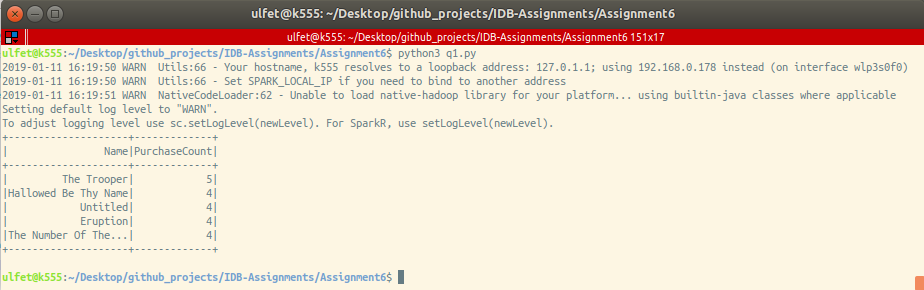
\includegraphics[scale=0.40]{spark_query.png}
			\caption{Spark Query Results}
			%\label{}
		\end{figure}
		\bigskip
		
		\bigskip
		\begin{figure}[H]
			\centering
			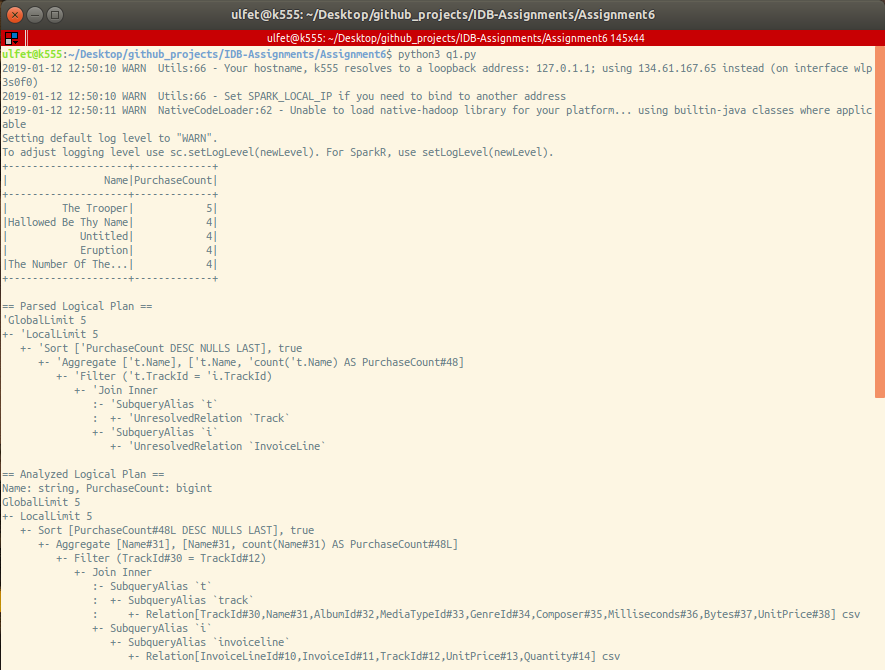
\includegraphics[scale=0.40]{all_plans_1.png}
			\caption{Spark Plans - Screenshot 1}
			%\label{}
		\end{figure}
		\bigskip
		
		In order to get all the related plans on Spark, we added a line of code to q1.py (our Spark runner given above):\\
		
		\begin{lstlisting}
		# run the query & display the answer
		sqlDF = spark.sql(queryText)
		sqlDF.show()
		sqlDF.explain(True)
		\end{lstlisting}
		
		
		
		\bigskip
		\begin{figure}[h]
			\centering
			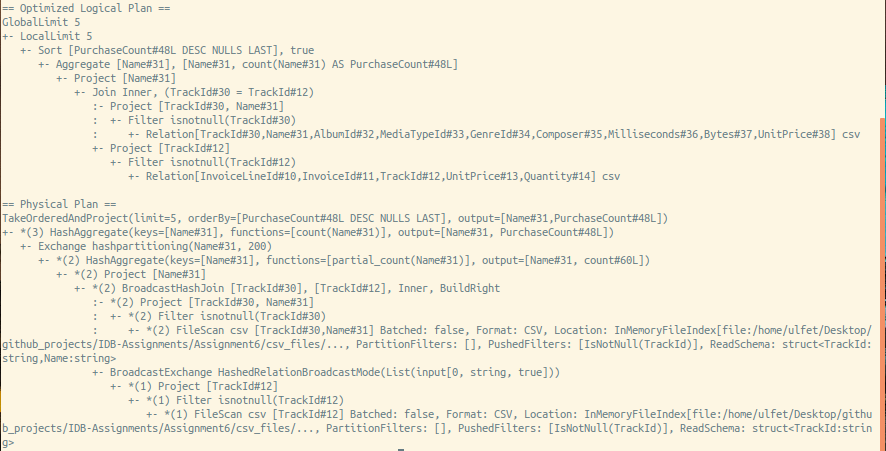
\includegraphics[scale=0.40]{all_plans_2.png}
			\caption{Spark Plans - Screenshot 2}
			%\label{}
		\end{figure}
		\bigskip	
		
		
		\clearpage
		
		\item Compare the query plans of Q5 by Spark and PostgreSQL (Exercise 1.2.5), and itemize the
		differences.
		
		\begin{comment}
			\bigskip
			\begin{figure}[h]
			\centering
			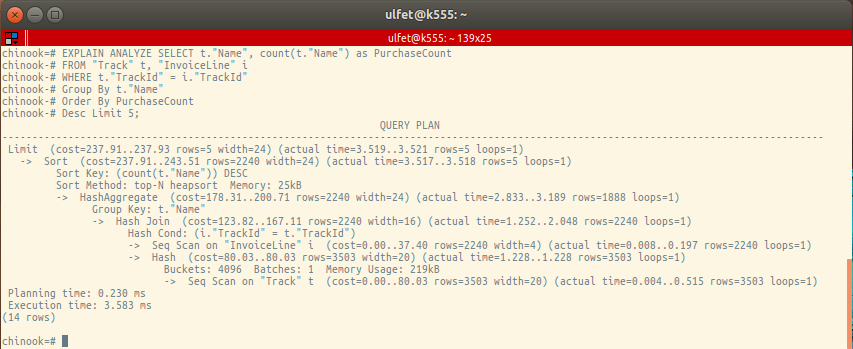
\includegraphics[scale=0.40]{compare_postgre_plan.png}
			\caption{Postgres Plan for Query}
			%\label{}
			\end{figure}
			\bigskip
			
			\bigskip
			\begin{figure}[h]
			\centering
			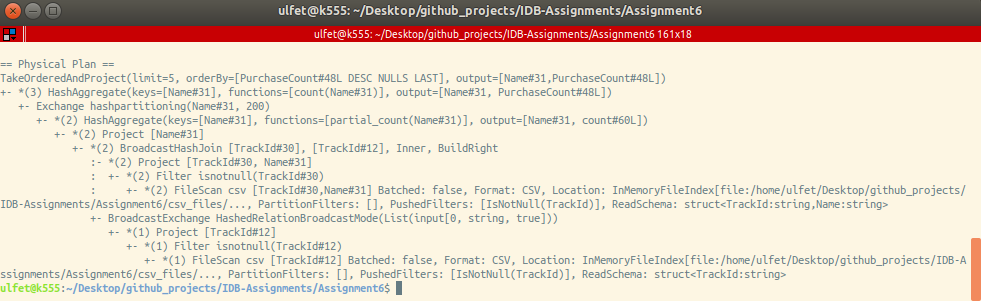
\includegraphics[scale=0.40]{compare_spark_plan.png}
			\caption{Spark Plan for Query}
			%\label{}
			\end{figure}
			\bigskip
		\end{comment}
		
		
		\bigskip
		\begin{figure}[H]
			\centering
			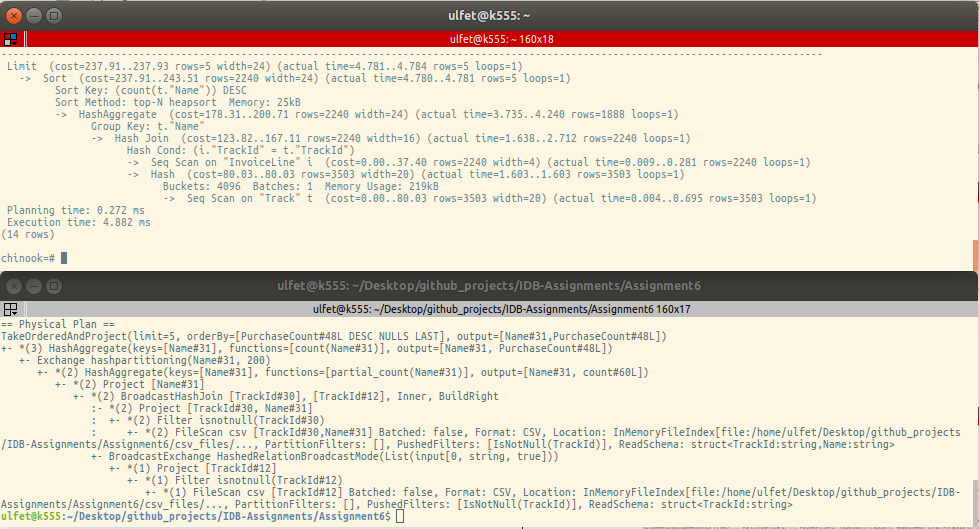
\includegraphics[scale=0.45]{compare_plans.png}
			\caption{Query Plan Comparison}
			%\label{}
		\end{figure}
		\bigskip
		
		\begin{comment}
			"SELECT t.Name, count(t.Name) as PurchaseCount \
			FROM Track t, InvoiceLine i \
			WHERE t.TrackId = i.TrackId \
			Group By t.Name \
			Order By PurchaseCount \
			Desc Limit 5"
		\end{comment}
		
		\bigskip
		Postgres' plan differs in the ways:
		\begin{itemize}
			\item Postgre starts with sequential scanning Track and hashing its rows into buckets.
			
			\item Then it sequential scans the InvoiceLine table and applies HashJoin on TrackId field(s) of those two tables.
			
			\item Then it groups the resulting combined rows on Track table's "Name" field and counts how many times a name has appeared.
			
			\item Finally, Postgre sorts the combined table on PurchaseCount and returns the first 5 rows (top 5 tracks).
		\end{itemize}
		\bigskip
		
		
		Spark's plan differs in the ways:\\
		\begin{itemize}
			\item Spark starts with scanning CSV file of InvoiceLine table, filters out rows that has their "TrackId" fields as null and projects <TrackId> values of rows. Then it broadcasts those TrackId values.
			
			\item Then, Spark, this time, scans CSV file of Track table, filters out rows that has their "TrackId" fields as null and projects <TrackId, Name> values of rows.
			
			\item Then it applies BroadcastHashJoin on TrackId fields of two resulting projection. On the resulting rows of BroadcastHashJoin, it projects <Name> values of rows.
			
			\item After that, Spark HashAggregates on "Name" field and counts how many times a specific name has appeared and names this count as PurchaseCount. Result of this step is rows containing <Name, PurchaseCount>
			
			\item Finally, Spark sorts the <Name, PurchaseCount> rows on "PurchaseCount" field, finds the greatest 5 rows, projects the "Name" field of those 5 rows as result.
		\end{itemize}
		
		
		
	\end{enumerate}
	
	
	
	
	
	\clearpage
	\subsection*{Exercise 6.2 (Datalog)}
	\begin{enumerate}
	    \item Given the following extensional database: 
	    \begin{enumerate}
	        \item teamNBA(X): X is a NBA basketball team 
	        \item coach(X,Y): X is a coach of team Y 
	        \item player(X,Y): X is a basketball player of team Y 
	        \item taller(X,Y): X is taller than Y. 
	    \end{enumerate}
	    Please formalize the following rules using Datalog and the given predicates (notably, there might be also non-NBA teams in 			this database):
	    \begin{enumerate}
	        \item  shorterTeammate(X,Y): X and Y are players in the same NBA basketball team, and X is shorter than Y.
	        \\Solution:
	        \\playersOfNBATeams(X,Y):-player(X,Y),teamNBA(Y)
	        \\shorterTeammate(X,Y):-playersOfNBATeam(X,Z),playersofNBATeam(Y,Z),taller(Y,X)
	        \item coachOrPlayer(X,Y): X is a coach or a player of a NBA basketball team Y.
	        \\Solution:
	        \\coachOrPlayer(X,Y):-coach(X,Y),teamNBA(Y)
	        \\coachOrPlayer(X,Y):-player(X,Y),teamNBA(Y)
	        \item coachTallest(X,Y): X is a coach of a NBA team Y, and X is taller than all the players in the team Y.
	        \\Solution:
	        \\Solution:
	        \\shorterCoachThanPlayer(X):-coach(X,Z),player(Y,Z),teamNBA(Z),taller(Z,X)
	        \\coachTallest(X,Y):-coach(X,Y),teamNBA(Y),NOT shorter(X)
	    \end{enumerate}
	    \item You have given the below facts F, rules R, and a query Q.
	    \begin{enumerate}
	        \item  Decide if the program given by the rules R is stratifiable. State why or why not it is stratifiable 					(corresponding graph with strati and statement).
	        \item Given the facts F and rules R do a fixpoint computation with all intermediate steps. Based on the computation, 				write down all answers to query Q. 
	        $
	        \\F: s(a,b) s(b,c) s(c,b) 
	            \\r(a) r(c) r(d)
            \\R: p(X,Y) \longleftarrow s(X,Y), NOT r(Y) 
                \\q(X,Y) \longleftarrow p(Y,X), s(X,Y) 
                \\q(X,Y) \longleftarrow q(Y,X), r(X) 
                \\t(X,Y) \longleftarrow r(X), q(X,Y)
            \\Q: t(X,Y)
            $

	    \end{enumerate}
	    Solution:
	    \begin{enumerate}
	        \item The given program is stratifiable because there is no negative predicate in the body of a recursive rule.
	        \\i.e. the rule $\\q(X,Y) \longleftarrow q(Y,X), r(X)$ has no negative dependency
	        \\ Or we can say that no two predicates of the same stratum depend negatively on each other as seen in the below graph
	        
	        
	        \bigskip
	        \begin{figure}[H]
	        	\centering
	        	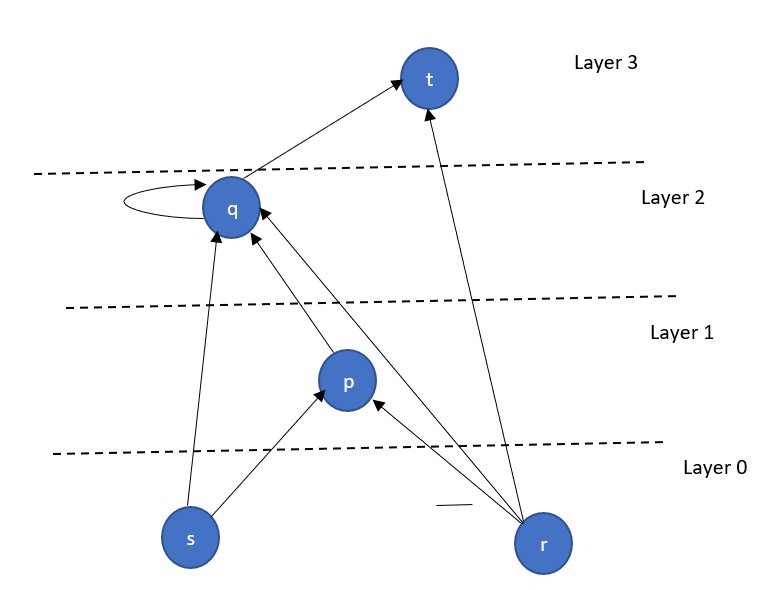
\includegraphics[]{dgraph.PNG}
	        	\caption{Query Plan Comparison}
	        	%\label{}
	        \end{figure}
	        \bigskip
	        
	        
	        \item Starting with F (F is all set of facts)
	        \begin{enumerate}
	        	\item Adding Td(F0)
	        	\\F1=F $\bigcup$ \{p(a,b),p(b,c)\}
	        	\item Adding Td(F1)
	        	\\F2= F $\bigcup$ \{p(a,b),a(b,c),q(b,c)\}
	        	\\F2= F $\bigcup$ \{p(a,b),a(b,c),q(c,b)\}
	        	\item Adding Td(F2)
	        	\\F3= F $\bigcup$ \{p(a,b),a(b,c),q(b,c),t(c,b)\}
	        	\\ Another application of Td(F3) yields the same result, therefore the least fixed point is reached.
	        \end{enumerate}
	        
	        
	        Answer of query q:t(X,Y) is (c,b)
	    \end{enumerate}
	\end{enumerate}
	
	\clearpage
	\subsection*{Exercise 6.3 (Data Integration)}
	Given is the following global schema with three relations:
	\\Hospital(HospitalName; Street;CityName; Postcode)
	\\Doctor(DoctorName;HospitalName;Disease)
	\\Patient(PatientName; Age; AttendingDoctorName)
	There are four data sources:
	
	One quick way is to do it manually for each bullet:
	
	\begin{description}
		\item[$\bullet$] DS1: AachenHospital(HospitalName, Street,Postcode): hospitals in Aachen.
		\item[$\bullet$] DS2: DoctorsAndPatients(DoctorName, PatientName, Disease): doctors and their patients.
		\item[$\bullet$]DS3: TeenagePatients(PatientName, Age): patient information with the patient age less
		than 18.
		\item[$\bullet$] DS4: Hospital(HospitalName, Street, Postcode, CityID), City(CityID, CityName, Country):
			hospitals and cities.
	\end{description}

	\begin{enumerate}
		\item Provide the LAV mappings between the source DS1 and the global schema.
		\item Provide the LAV mappings between the source DS2 and the global schema.
		\item For DS3 and the global schema, which mapping is more precise, a GAV mapping or a LAV
		mapping? Why? Also provide the mapping you think is more precise.
		\item Consider DS4 and the global schema. Rewrite the below query on the global schema to a
		query on the schema of DS4. 
		\\q(CityName) :- Hospital('FrancisHospital';-;CityName; ):
	\end{enumerate}
	Solution: 
	\begin{enumerate}
		\item AachenHospital(HospitalName, Street, PostCode):-
		\\Hospital(HospitalName,Street,CityName,PostCode),\\ CityName='Aachen'
		\item DoctorsAndPatients(DoctorName,PatientName,Disease):-
		\\Doctor(DoctorName,\_,Disease),
		\\Patient(PatientName,\_,AttendingDoctorName)
		\item LAV:\\ TeenagePatients(PatientName,Age):-
		\\Patient(PatientName,Age,\_), Age<18
		\\ \\GAV:\\Patient(PatientName,Age,AttendingDoctorName):-
		\\DoctorsAndPatients(DoctorName,PatientName,\_),
		\\TeenagePatients(PatientName,Age)
		\\ \\Here LAV mapping is more precise, because in GAV mapping the Age does not map to patients who are older than 18 years. Here Source centric Mapping is used (As constraint is on source level). But global schema does not define any constraint.
		\item q'(CityName):- Hospital('FrancisHospital',\_,\_,CityID), City(CityID,CityName,\_)
	\end{enumerate}
	
	\clearpage
	\subsection*{Exercise 6.4 (Answer questions briefly)}
	\begin{enumerate}
	    \item What is the goal of systems like Pig Latin or Hive?
	    \item When do you need to do shuffling in Spark? What are narrow and wide dependencies?
	    \item Sketch a data integration architecture. What is a mediator? What is the task of a mediator in a data integration 			architecture?
	    \item What is the Herbrand Base and the Herbrand Model?
	\end{enumerate}
	Solution:
	\begin{enumerate}
	    \item The main goal of high level languages like pig or hive is to reduce the workload of the user by preventing the need of 			writing complex map-reduce jobs in java. Pig uses a procedural style approach and hive uses a SQL style approach 			which makes data manipulation of Hadoop data easy.
	    \item We need shuffling in spark i.e. distribution of RDD between different nodes of a cluster when the operation can't be 			performed within a single partition. Examples of such operations are join,distinct,groupByKey.
	    \\When a partition is dependent of one or two parent partitions it is called as "Narrow dependencies".However,when a 			partition is dependent on multiple parent partitions it is termed as "wide dependencies".
	    \item
	     A mediator maintains a global schema and mappings between the global and source schemas. It is the task of the mediator to consult the mappings to decide which data to retrieve from the sources and how to combine them appropriately in order to form the answer to the user’s query.
	     \bigskip
	     \begin{figure}[H]
	     	\centering
	     	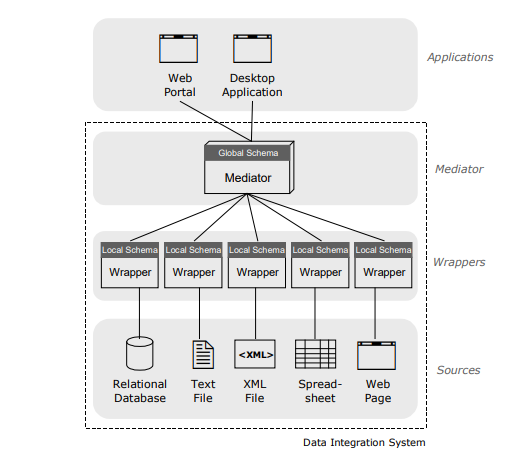
\includegraphics[scale=0.40]{Data_integration.png}
	     	\caption{Data Integration System Architecture}
	     	%\label{}
	     \end{figure}
	     \bigskip

	    \item
	    Herbrand Base of D: All positive ground literals are constructable from predicates in D and constants in D.
	    \\Herbrand Model of D:A Herbrand Model is every subset M of the Herbrand Base of D, such that:
        \\Every fact from F is contained in M. For every ground instance of a rule in D over constants in D, if M contains all literals 	in the body, then M contains the head as well.
        \\A minimal model does not properly contain any other model
	\end{enumerate}
	
\end{document} 
